\subsection{Márvány padlón helyben forgás}
A \ref{fig:Left_n50Right50Aulaa} megfigyelhető, amint a robot márvány padlón differenciálisan fordul 50 másodpercen keresztül, ezalatt háromszor teljen körbefordul. A pályát tekintve a robot központja elmozdul, az X és a Y tengelyen is.  Az oldalirányú mozgás a nem egyenlő súrlódási erők miatt jön létre.
A fordulás közben a kerekek követik az előírt referencia szögsebességeket, amint az \ref{fig:Left_n50Right50Aulax} ábrán is látható.
A fordulási szögsebesség 25 \degree/s, nagyobb, mint a \ref{fig:Left_n50Right50d}, mivel nagyobb referencia értékek íródtak elő a kerekeknek.

A szabályzók működése közben a kitöltési tényező hullámzik mind a négy kerék esetében, ami a többi mérés esetében nem fordult elő.

\renewcommand{\nth}{2}
\renewcommand{\GlobalPath}{Meresek/AulaMeresek/JobraDiff_Aula_07/}
\renewcommand{\secondImage}{*}



\begin{figure}[H]
  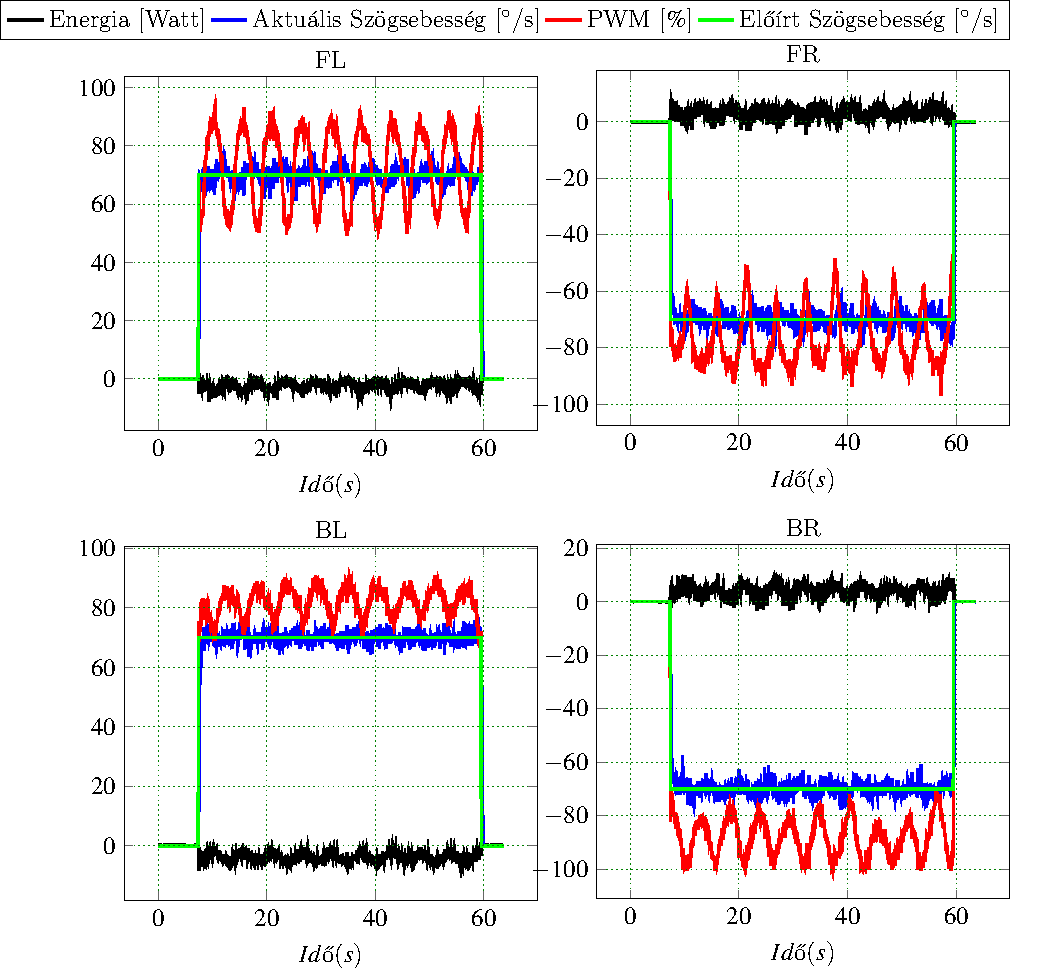
\includegraphics{tikz/Left_n50Right50Aulax.pdf}
  \caption{$SSMR-4W$ típusú robot mozgása, tengelyekre bontva, ha a kerék szögsebességek BL=FL=70\degree/s és a FR=BR=-70\degree/s}
  \label{fig:Left_n50Right50Aulax}
\end{figure}


\begin{figure}[H]
  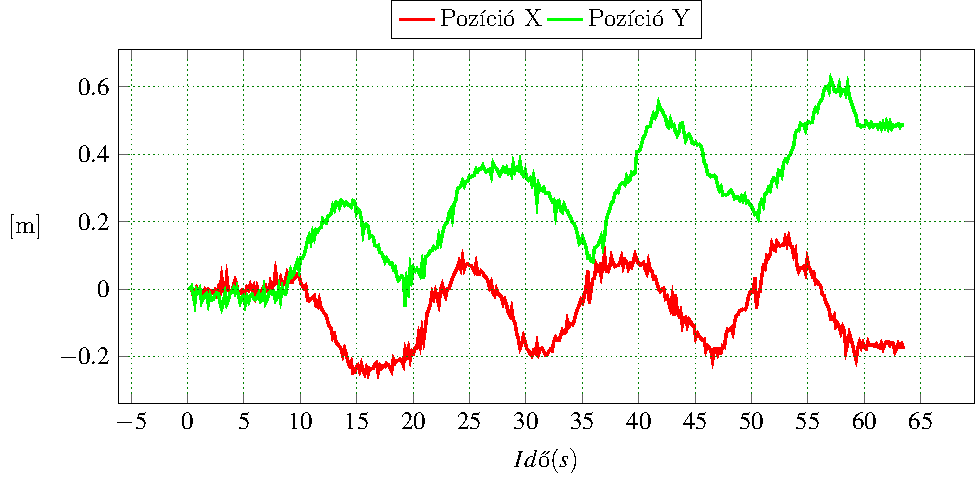
\includegraphics{tikz/Left_n50Right50Aulaa.pdf}
  \caption{$SSMR-4W$ típusú robot mozgása, ha a kerék szögsebességek BL=FL=70\degree/s és a FR=BR=-70\degree/s}
  \label{fig:Left_n50Right50Aulaa}
\end{figure}


\begin{figure}[H]
  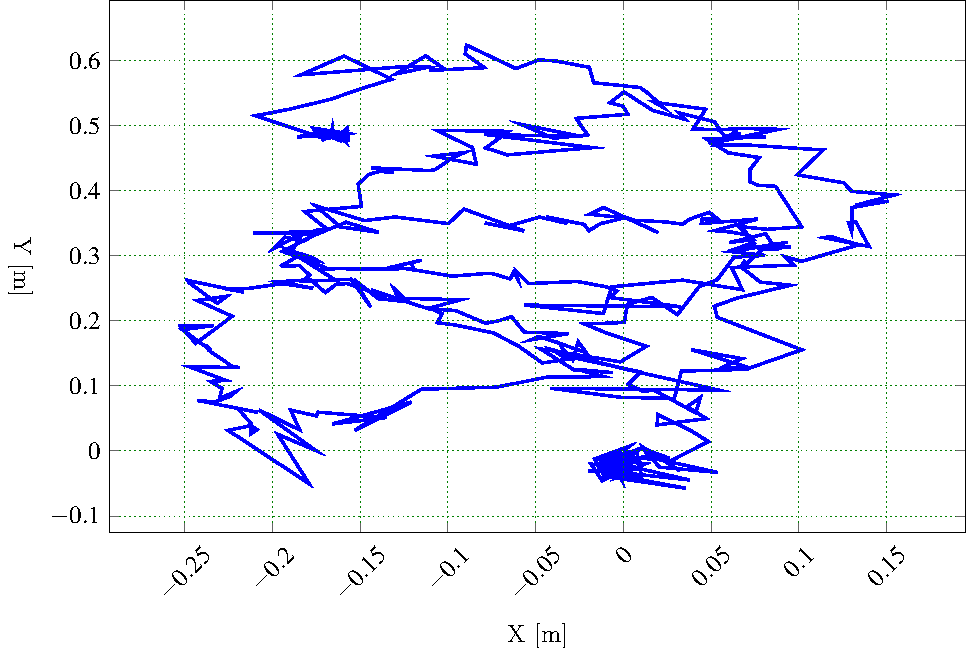
\includegraphics[scale=1]{tikz/Left_n50Right50Aulab.pdf}
  \caption{$SSMR-4W$ típusú robot által leírt pálya, ha a kerék szögsebességek BL=FL=70\degree/s és a FR=BR=-70\degree/s}
    \label{fig:Left_n50Right50Aulab}
\end{figure}



\begin{figure}[H]
  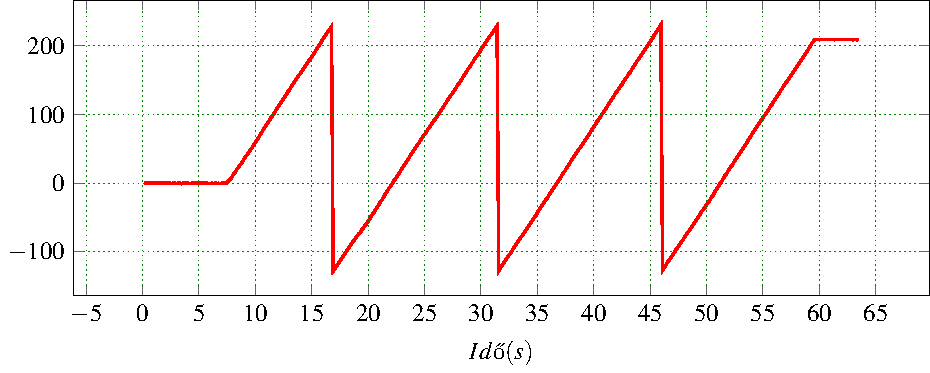
\includegraphics{tikz/Left_n50Right50PAulac.pdf}
  \caption{$SSMR-4W$ típusú robot orientációja,  ha a kerék szögsebességek BL=FL=70\degree/s és a FR=BR=-70\degree/s}
    \label{fig:Left_n50Right50PAulac}
\end{figure}

A \ref{fig:Left_n50Right50Aulad} megfigyelhető, hogy a LIDAR által mért szögsebesség sokkal kevésbé zajos, mint \ref{fig:Left0Right50d}, amiatt, hogy a márvány padló sokkal egyenesebb, mint a kavicsos talaj, így nincsenek jelen kisebb-nagyobb bukkanok, amik zajforrásként jelenek meg a LIDAR térképezés számára.

\begin{figure}[H]
  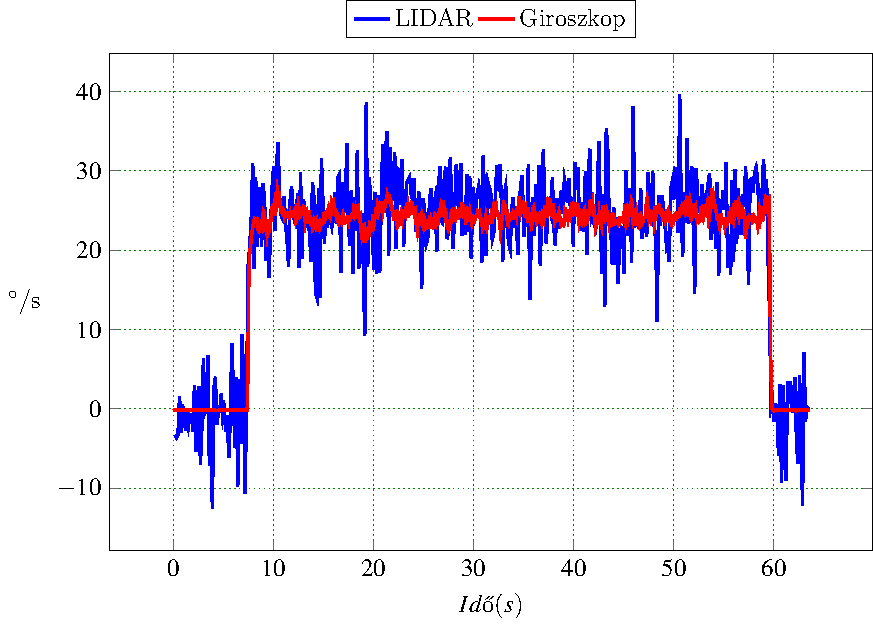
\includegraphics{tikz/Left_n50Right50Aulad.pdf}
  \caption{$SSMR-4W$ típusú robot fordulási szögsebessége Z tengely körül, ha a kerék szögsebességek BL=FL=70\degree/s és a FR=BR=-70\degree/s}
    \label{fig:Left_n50Right50Aulad}
\end{figure}
